\documentclass[10pt]{beamer}

\usepackage{arev}
\usepackage[sfdefault]{FiraSans}
\usepackage{inconsolata}
\usepackage{graphicx}
\usepackage{listings}
\usepackage{xcolor}
\lstset{basicstyle=\ttfamily,language=Java}

\definecolor{blackish}{RGB}{56,58,54}
\definecolor{redish}{RGB}{109,41,49}
\definecolor{red}{RGB}{152,41,50}
\definecolor{orangeish}{RGB}{188,71,0}
\definecolor{blueish}{RGB}{25,33,139}

\setbeamercolor{structure}{fg=redish}
\setbeamercolor{frametitle}{fg=redish}
\setbeamercolor{title}{fg=blackish}
\setbeamercolor{itemize item}{fg=redish}
\setbeamercolor{itemize subitem}{fg=redish}
\setbeamertemplate{itemize item}[triangle]
\setbeamertemplate{itemize subitem}[triangle]

\setbeamertemplate{frametitle}{\vskip1em\insertframetitle\par\vskip0.5em}

\setbeamertemplate{footline}{%
  \hbox{%
    \begin{beamercolorbox}[wd=0.45\paperwidth,ht=2.5ex,leftskip=0.4cm,dp=1ex]{footline}%
      \color{red} COMP2000: Object Oriented Programming Practices
    \end{beamercolorbox}%
    \begin{beamercolorbox}[wd=0.45\paperwidth,ht=2.5ex,rightskip=0.4cm,dp=1ex]{footline}%
      \hfill
\includegraphics[height=1ex]{../logo.jpg}
    \end{beamercolorbox}%
  }%
}

\title{\color{redish} COMP2000 Week 8: Patterns 2}
\subtitle{Decorator, Iterator, State}
\date{}

\begin{document}

\begin{frame}
\titlepage
Three patterns, one story: all three are \textbf{composition plus delegation}, and all three serve the Open/Closed Principle.  Working code is left untouched; behaviour is added from outside.
\begin{itemize}
  \item Preparation: \textit{Head First Design Patterns} ch.\ 3, 9 (Iterator section only), 10
  \item Next week's EPIC: a public debate on design patterns, argued against another team's code
\end{itemize}
\end{frame}

% ---------------------------------------------------------------- Decorator
\begin{frame}{Decorator: the intent}
\begin{center}
\begin{beamercolorbox}[sep=0.8em,wd=\textwidth]{block body}
\emph{Attach additional responsibilities to an object dynamically, without changing its class, by wrapping it.}
\end{beamercolorbox}
\end{center}
\end{frame}

\begin{frame}{Decorator}
\begin{center}
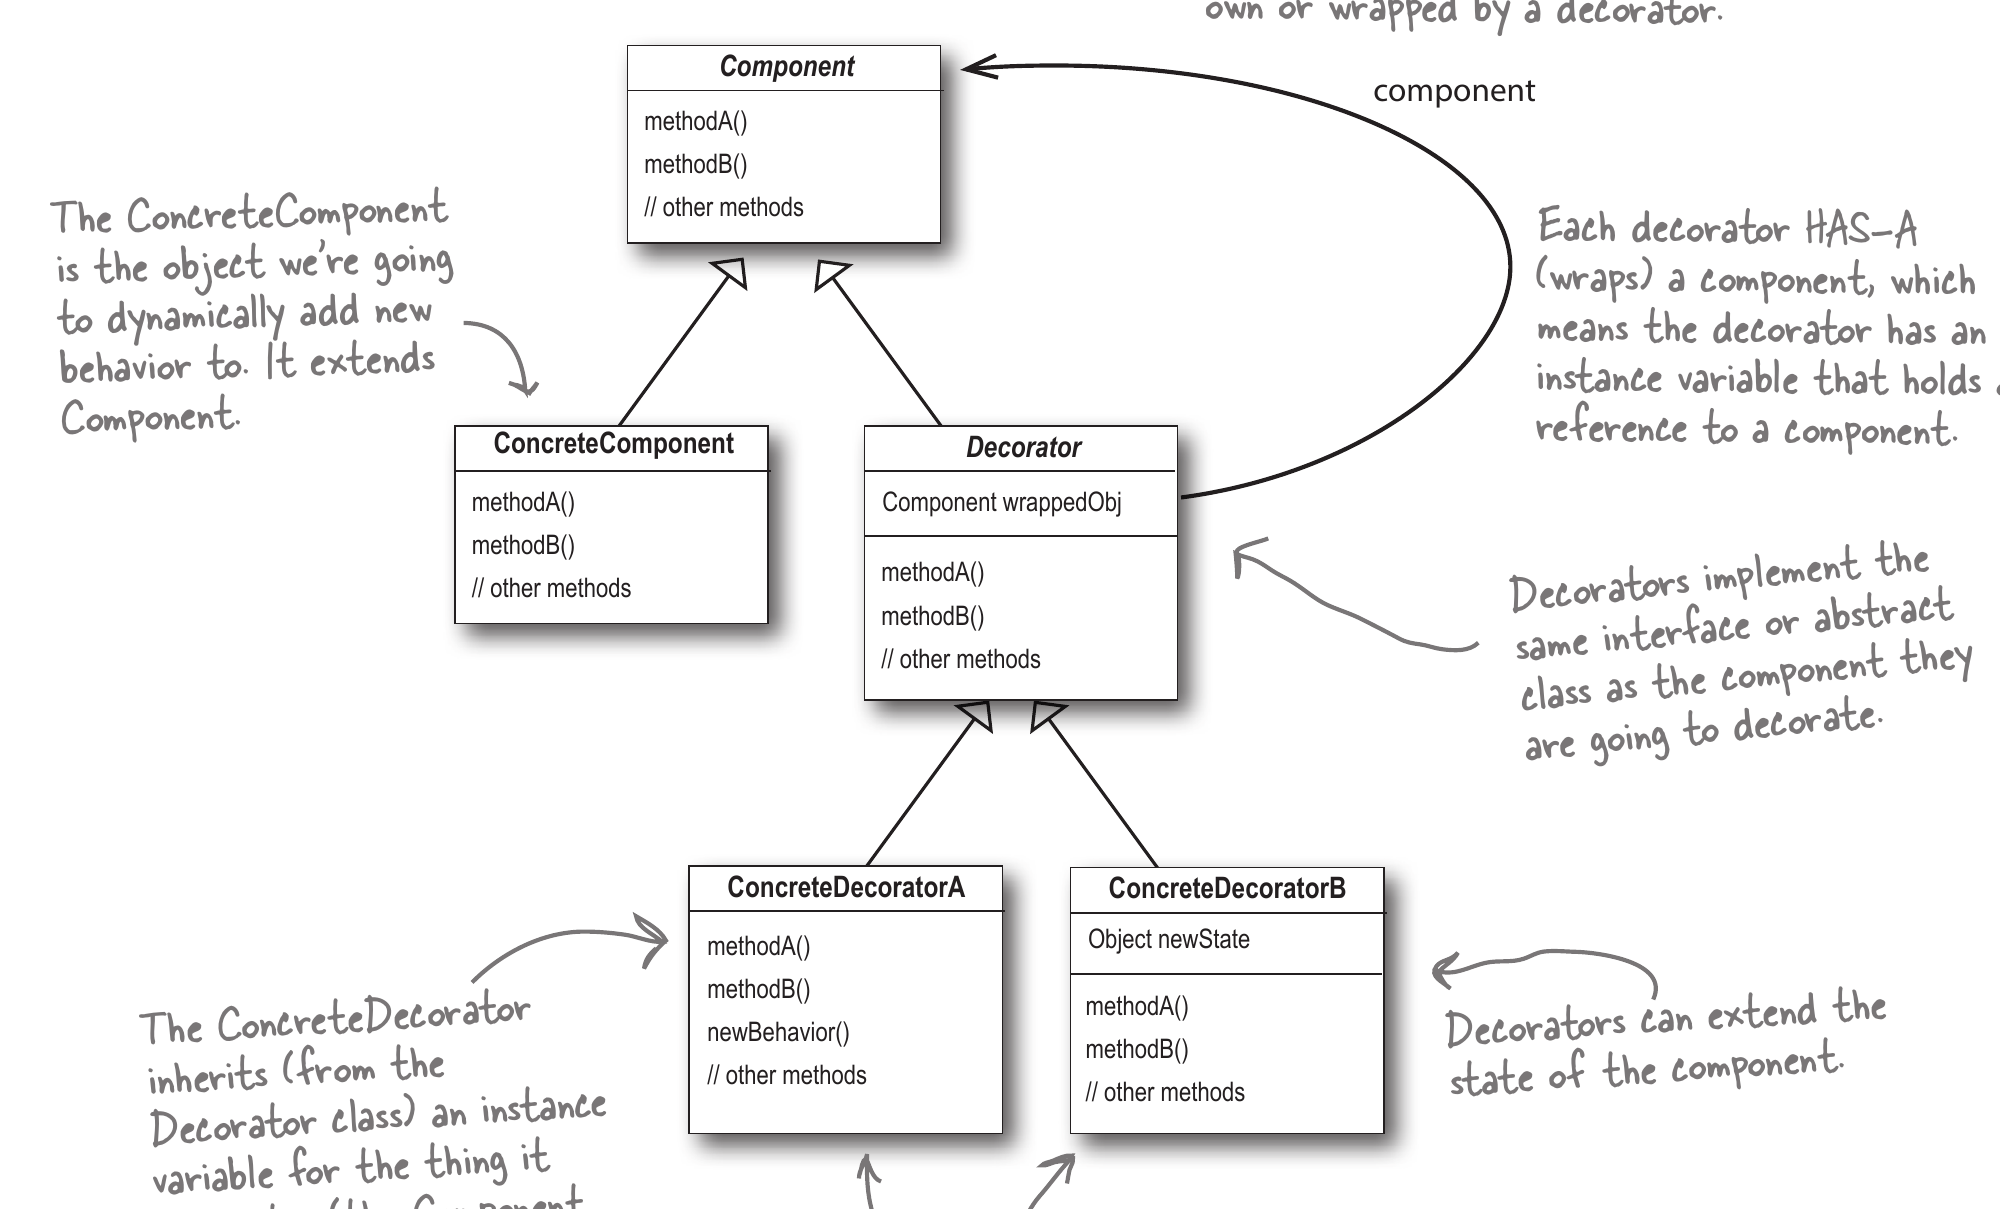
\includegraphics[width=\textwidth,height=0.78\textheight,keepaspectratio]{figures/decorator-pattern.png}
\end{center}
\end{frame}

\begin{frame}{Decorator: the takeaway}
\begin{center}
\begin{beamercolorbox}[sep=0.8em,wd=\textwidth]{block body}
\emph{The pattern is a recursive data type wearing a costume: the inheritance only buys type compatibility, so a decorator can substitute for the thing it wraps, while the aggregated reference does all the real work, and the whole stack bottoms out in a genuine component, because you cannot decorate something that does not exist.}
\end{beamercolorbox}
\end{center}
\end{frame}

% ---------------------------------------------------------------- Iterator
\begin{frame}{Iterator: the intent}
\begin{center}
\begin{beamercolorbox}[sep=0.8em,wd=\textwidth]{block body}
\emph{Provide a way to access a collection's elements sequentially without exposing how it is stored.}
\end{beamercolorbox}
\end{center}
\end{frame}

\begin{frame}{Iterator}
\begin{center}
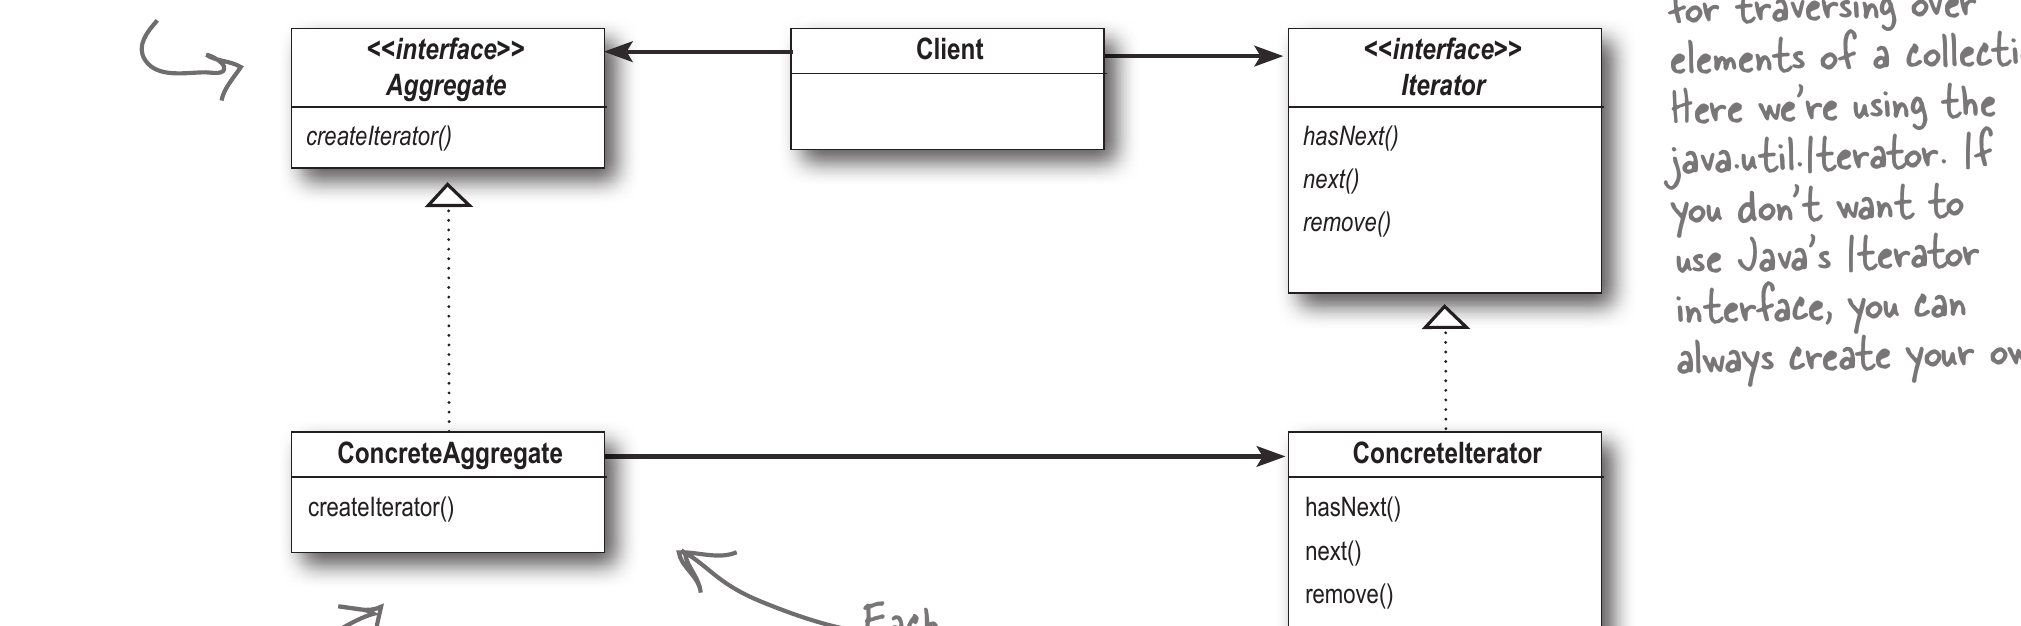
\includegraphics[width=\textwidth,height=0.78\textheight,keepaspectratio]{figures/iterator-pattern.png}
\end{center}
\end{frame}

\begin{frame}{Iterator: the takeaway}
\begin{center}
\begin{beamercolorbox}[sep=0.8em,wd=\textwidth]{block body}
\emph{It is the ``give me your iterator'' relationship rather than ``you are an iterator'': the iterator is a separate object carrying its own position, and \texttt{Iterable} is only the socket (three methods, one abstract) that the enhanced for loop is compiler sugar over, so \texttt{forEach()} and arrays can both side-step the pattern entirely while still looking like they are using it.}
\end{beamercolorbox}
\end{center}
\end{frame}

% ---------------------------------------------------------------- State
\begin{frame}{State: the intent}
\begin{center}
\begin{beamercolorbox}[sep=0.8em,wd=\textwidth]{block body}
\emph{Let an object change its behaviour when its internal state changes, so it looks like it changes class.}
\end{beamercolorbox}
\end{center}
\end{frame}

\begin{frame}{State}
\begin{center}
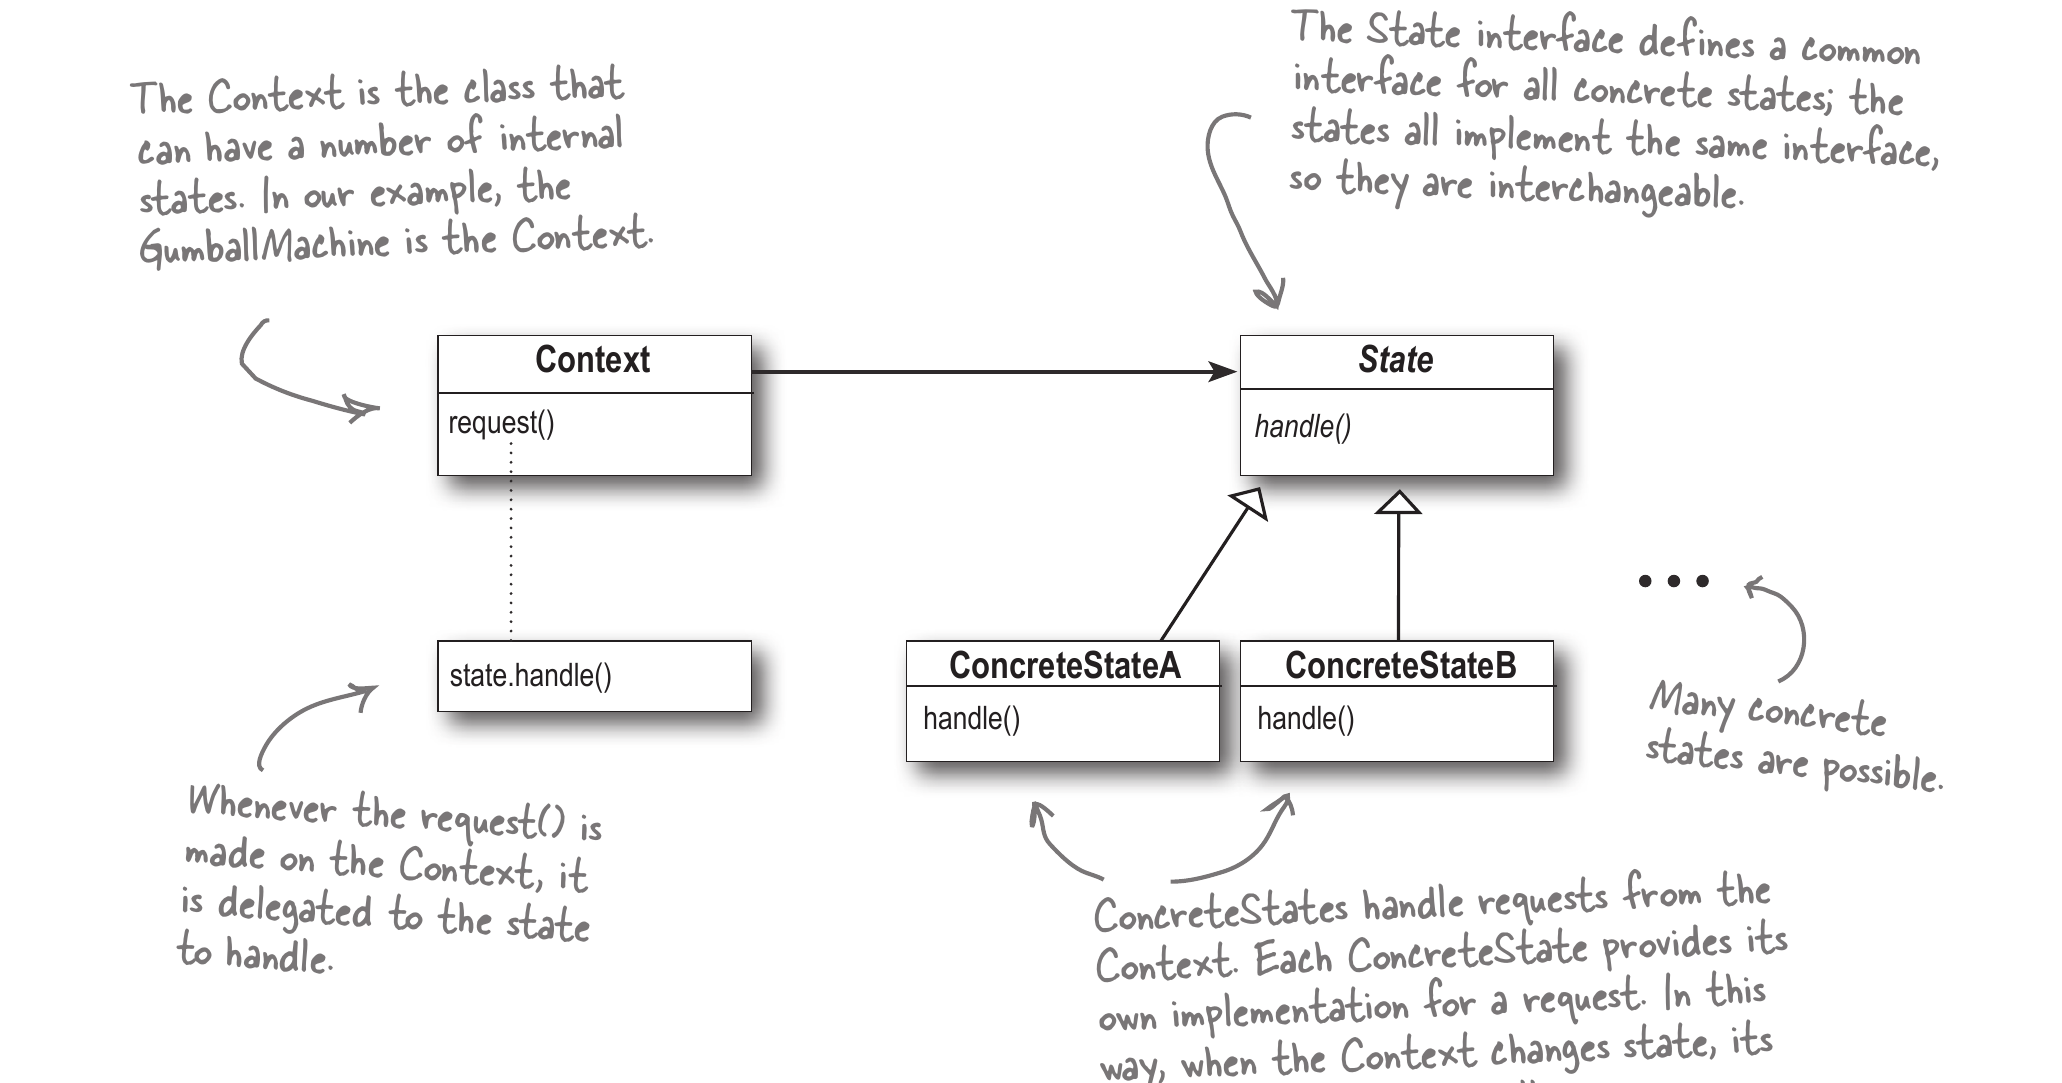
\includegraphics[width=\textwidth,height=0.78\textheight,keepaspectratio]{figures/state-pattern.png}
\end{center}
\end{frame}

\begin{frame}{State: the takeaway}
\begin{center}
\begin{beamercolorbox}[sep=0.8em,wd=\textwidth]{block body}
\emph{Unlike Strategy, each state must know its context, because it has to transition it; that bounded coupling is the whole point, and the interesting design choice is whether states build the next state themselves, or the context owns all of them so that a state's fields can survive a transition.}
\end{beamercolorbox}
\end{center}
\end{frame}

\end{document}
